\documentclass[12pt,a4paper,twopage]{article}
\usepackage[utf8]{inputenc}
\usepackage[a4paper,margin=1cm,footskip=.5cm]{geometry}
\usepackage{multicol}
\usepackage{amsmath}
\usepackage{float}
\usepackage{epsfig,graphicx}
\usepackage{xcolor,import}
\usepackage{subcaption}
\usepackage[font=small,labelfont=bf]{caption}
\usepackage{siunitx}
\usepackage[german]{babel}
\usepackage{textcomp}
\usepackage{mathtools}
\linespread{1.1}
\usepackage{parskip}
\setlength{\parindent}{12pt}

\begin{document}


\thispagestyle{empty}
			\begin{center}
			\Large{Fakultät für Physik}\\
			\end{center}
\begin{verbatim}


\end{verbatim}
							%Eintrag des Wintersemesters
			\begin{center}
			\textbf{\LARGE SOMMERSEMESTER 2015}
			\end{center}
\begin{verbatim}


\end{verbatim}
			\begin{center}
			\textbf{\LARGE{Physikalisches Praktikum II}}
			\end{center}
\begin{verbatim}




\end{verbatim}

			\begin{center}
			\textbf{\LARGE{PROTOKOLL}}
			\end{center}
			
\begin{verbatim}





\end{verbatim}

			\begin{flushleft}
			\textbf{\Large{Experiment (Nr., Titel):}}\\
							%Experiment Nr. und Titel statt den Punkten eintragen
			\LARGE{11: Hall-Effekt}	
			\end{flushleft}

\begin{verbatim}

\end{verbatim}	
							%Eintragen des Abgabedatums, oder des Erstelldatums des Protokolls
			\begin{flushleft}
			\textbf{\Large{Datum:}} \Large{12.06.2015}
			\end{flushleft}
			
\begin{verbatim}
\end{verbatim}
							%Namen der Protokollschreiber
		\begin{flushleft}
			\textbf{\Large{Bachleitner Veronika, Grafendorfer Erik}} 
			\end{flushleft}

\begin{verbatim}


\end{verbatim}
							%Kurstag und Gruppennummer, zb. Fr/5
			\begin{flushleft}
			\textbf{\Large{Kurstag/Gruppe:}} \Large{FR/1}
			\end{flushleft}

\begin{verbatim}






\end{verbatim}
							%Name des Betreuers, das Praktikum betreute.
			\begin{flushleft}
			\LARGE{\textbf{Betreuer:\Large{ KLEPP }}}		
			\end{flushleft}
			
\pagebreak			
			
\section{Aufgabenstellung}
Wir untersuchen verschiedene Größen die beim Halleffekt in Halbleitern auftreten.
\section{Theorie}
In Magnetfeldern wirkt auf bewegte Ladungen eine Kraft (Lorentz-Kraft) senkrecht zu ihrer Bewegungsrichtung:
$$F_L=q(\vec{E}+\vec{v}\times \vec{B})$$
In einem stromdurchflossenen Leiter "schiebt" diese Kraft die Ladungsträger auf eine Seite des Leiters, und es kommt zu einer Ladungstrennung. Dieses Phänomen nennt man \textit{Hall-Effekt}.\\
Diesen Effekt kann man nutzen, um das Vorzeichen und die Anzahldichte der Ladungsträger in einem Leiter zu bestimmen oder um Magnetfeldstärken zu messen.\\
Die Potentialdifferenz zwischen dem oberen und dem unteren Rand des Streifens (Leiters) nennt man \textit{Hall-Spannung}. Ihren Wert können wir als Funktion der Driftgeschwindigkeit der Ladungsträger angeben. Das Magnetfeld übt auf die Ladungsträger im Streifen eine Kraft $q v_d B$ aus, die kompensiert wird durch die elektrostatische Kraft $-q E_H$. $E_H$ ist das elektrische Feld, das durch die Ladungstrennung im Leiter entsteht. Der Gleichgewichtszustand ist also $E_H=v_d B$. Ist die Breite des Streifens gleich $b$, so beträgt die Potentialdifferenz $E_H b$. Daher ist die Hall-Spannung gegeben durch: \footnote{Physik für Wissenschaftler und Ingenieure, Paul A. Tipler, Gene Mosca, 6. Auflage, Kapitel 26.4}
$$U_H=E_H b = v_d B b$$

Aus der Längsspannung am Halbleiter und dem Strom durch ihn ergibt sich der Widerstand R des Leiters.

Aus R ergeben sich mit der Länge l und der Fläche A des Leiters der spezifische Widerstand $\rho$ und die Leitfähigkeit $\sigma$:

$$ R = \rho \frac{l}{A} $$

$$ \sigma = \frac{1}{\rho} $$
Die Leitfähigkeit kann auch durch die Dichte der Ladungsträger $n$, ihre Ladung $q$ und ihre Beweglichkeit $\mu$ berechnet werden:
$$ \sigma = n \cdot q \cdot \mu $$

Damit ergeben sich für $\sigma$ und $\mu$ :

$$ \sigma = \frac{1}{R} \frac{l}{A} $$

$$ \mu = \frac{\sigma}{n \cdot q} $$

Die Dichte der Ladungsträger $n$ erhalten wir aus der Hall-Konstante:

$$ n = -\frac{1}{q\cdot R_H} $$

Wobei q die Elementarladung bedeutet.

\subsubsection*{Hall-Spannung:}
Oben haben wir bereits eine Formel für die Hall-Spannung definiert: $U_H=v_d B b$. Diese können wir umschreiben, sodass nur solche Größen vorkommen, die in unserem Aufbau bekannt sind oder gemessen werden können.\\
Mit $v_d=\mu \vec{E}=\frac{\mu}{\sigma}\vec{j}$ erhalten wir $U_H=\frac{\mu}{\sigma}\vec{j} B b$.\\
Der Strom $I$ ist gleich der Stromdichte $\vec{j}$ durch die Fläche $\Rightarrow \vec{j} \cdot b = I/d$ mit der Dicke der Probe $d$. Setzen wir nun noch für die Leitfähigkeit $\sigma=n \cdot q \cdot \mu$ ein erhalten wir: 

$$U_H=\frac{1}{nq} \frac{I \cdot B}{d}=R_H \frac{I \cdot B}{d}$$

Der lineare Fit durch den Plot der Hallspannung gegen die variierte Probenstromstärke $I_{Probe}$ ergibt einen Fitparameter $\alpha$, aus dem wir einen ersten Wert für $R_H$ erhalten:

\begin{equation}
\label{afit}
\begin{split}
U_H(I_{Probe})& = \alpha I \\
U_H(I_{Probe})& = \frac{R_H B}{d} I \\
\rightarrow \alpha & = \frac{R_H B}{d} \\
\rightarrow R_H & = \frac{\alpha d}{B}
\end{split}
\end{equation}

Der lineare Fit durch den Plot der Hallspannung in Abhängigkeit der magnetischen Flussdichte liefert uns einen Parameter $\beta$, der sich wie folgt darstellt:

\begin{equation}\label{bfit}
\begin{split}
U_H(B)& = R_H \frac{I B}{d} \\
U_H(B)& = \beta B \\
\rightarrow \beta & = \frac{I R_H}{d} \\
\rightarrow R_H & = \frac{\beta d}{I}
\end{split}
\end{equation}



\section{Aufbau}
Wir haben ein Hall-Effekt-Grundgerät zur Verfügung gestellt, außerdem einen Elektromagneten sowie zwei Multimeter. Eine Computer-Schnittstelle und ein entsprechendes Messprogramm helfen, die Temperaturabhängigkeit des Hall-Effekts zu messen.\\
Wir haben je ein Grundgerät für n-Ge und p-Ge, an denen alle notwendigen Kontakte für Messungen und Versorgungsspannungen angebracht sind.

\section{Durchführung}
Aus der relativen Unsicherheit des Abstandes zwischen den Polschuhen ($\frac{\Delta d}{d}= \frac{0.2}{10} = 0.02 $ erhalten wir auch die relative Unsicherheit des B-Feldes:  0.02. Dazu kommt aber noch die Unsicherheit durch die Erzeugung des B-Feldes mit dem Netzgerät, die $\pm$ 1 mA beträgt - und die relative Unsicherheit der Relation zwischen der erzeugenden Stromstärke des B-Feldes, die $\frac{0.25 T}{48.7 mA}$ beträgt. In den Plots und den Fits wurden alle berücksichtigt. 

Für die Unsicherheit der Hallspannung wurde nur die Digitalisierungsunsicherheit des Multimeters berücksichtigt. 

Für zusammengesetzte Unsicherheiten wurde die Gaußsche Fehlerfortpflanzung angewandt.
\section{Ergebnisse}
\subsection*{Messungen bei konstantem Magnetfeld}

\begin{figure}
\begin{center}

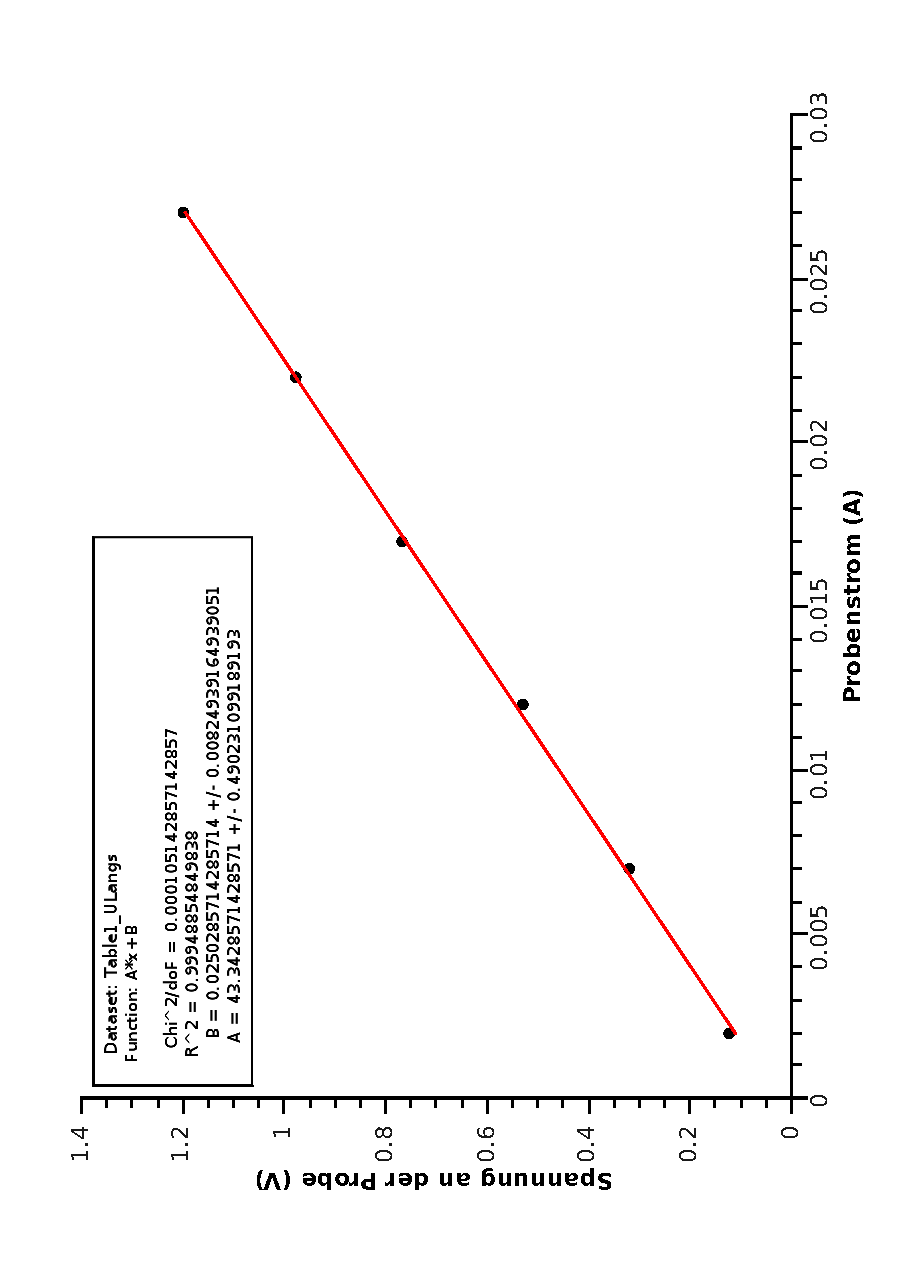
\includegraphics[width=0.4\linewidth, angle=-90]{widerstand.eps}
\caption{Widerstandsbestimmung durch linearen Fit\label{widerstandimg}}
\end{center}
\end{figure}

Aus dem linearen Fit in \textbf{Abb. (\ref{widerstandimg})} durch die Längsspannung in Abhängigkeit des Probenstroms ergibt sich direkt der Widerstand des Halbleiters als Steigung der Gerade:

\begin{center}


$$\boxed{R_n =  (43.3 \pm 0.5) \Omega }$$

Mit $ R_n = \rho_n \frac{l}{A} $ , wobei $\frac{l}{A}$ hier 2000 $m^{-1}$ sind:

$$\rho_n = (0.02165 \pm 0.00025) \Omega m^{-1} $$
$$\boxed{\sigma_n =  (46.2 \pm 0.6) \Omega^{-1}m^{-1} }$$  

\end{center}

qtiplot gibt für den Fit in \textbf{Abb. (\ref{hallspkonst})}  $\alpha$:

$$ \alpha = 1.88 \pm 0.05 $$

Daraus mit (\ref{afit}) nach $R_H$:

\begin{center}
$$ \boxed{ R_H(I_{Probe}) = (0.0125 \pm 0.0006) \frac{m^3}{As} } $$
\end{center}

Daraus ergibt sich für n:

\begin{center}
$$ \boxed{ n_{IProbe} = (5.0 \pm 0.3) \cdot 10^{20} m^{-3} } $$
\end{center}


\begin{figure}
\begin{center}
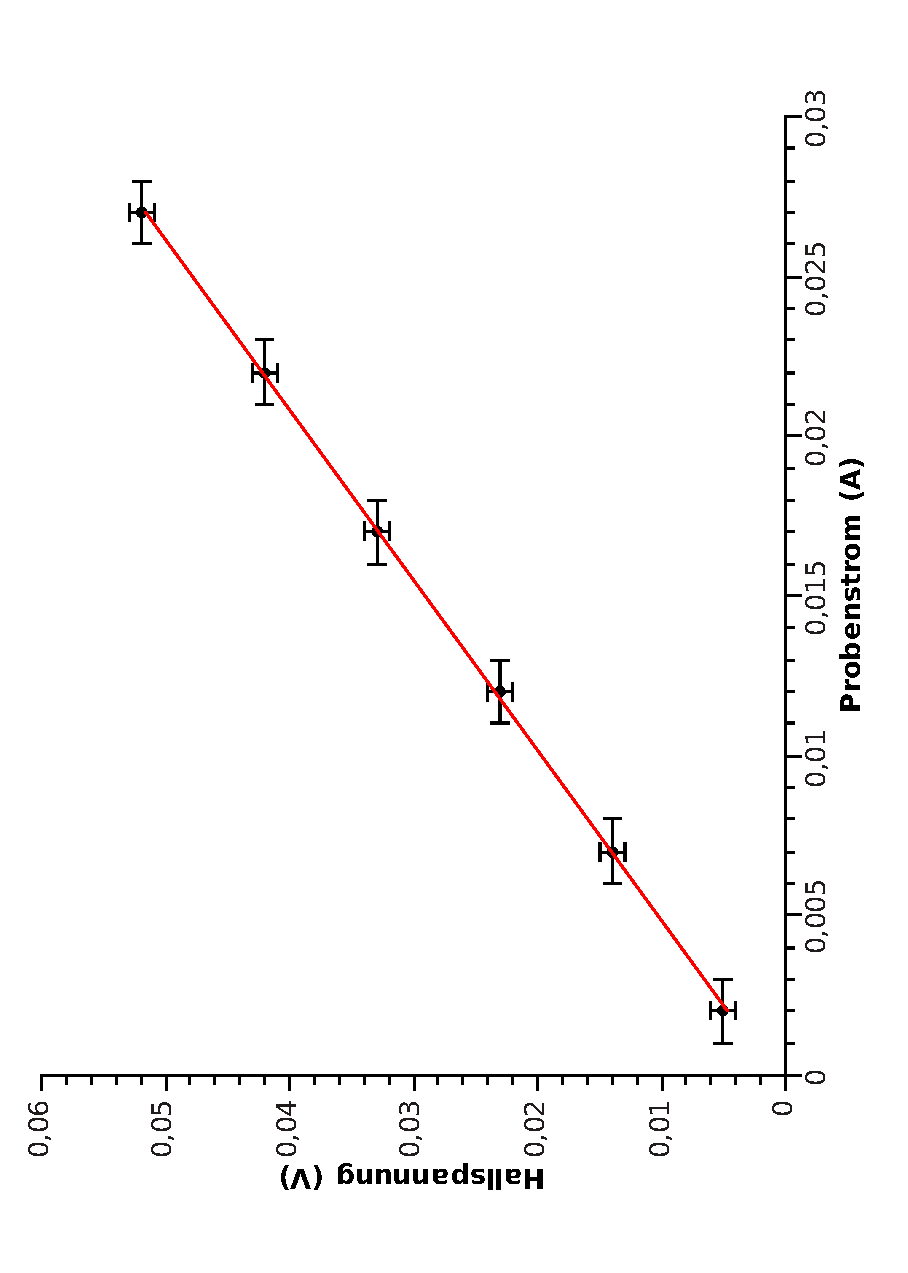
\includegraphics[width=0.4\textwidth, angle=-90]{hallkonst.eps}
\caption{Probenstromabhängige Hallspannung \label{hallspkonst}}
\end{center}
\end{figure}

\subsection*{Hallkonstante an n-Germanium}

Laut (\ref{bfit}) gibt qtiplot für $\beta$ in \textbf{Abb. (\ref{hallbimg})}:

$$ \beta = \frac{I R_H}{d} =  0.206 \pm 0.006 $$

Daraus erhalten wir mit (\ref{bfit}) für $R_H$:

\begin{center}
$$ \boxed{ R_{H} = \frac{\beta d}{I} = (0.0082 \pm 0.0005 )  \frac{m^3}{As}  } $$
\end{center}

\begin{center}
$$ \boxed{ n_{n} = q \cdot R_H = (7.6 \pm 0.5) \cdot 10^{20} m^{-3}  } $$
\end{center}

$$\boxed{ \mu_n = (0.38 \pm 0.03) \frac{m^2}{Vs} } $$

\subsection*{Hallkonstante an p-Germanium}
Mit der selben Methode, durch lineare Fits in \textbf{Abb. (\ref{hallbimg})}, erhalten wir für $R_H$ an p-Ge:

$$ \text{Fitparameter } \beta = 0.25 \pm 0.01 $$

$$\rho_p = \frac{58.2}{2000} = (0.029 \pm 0.002) \Omega m^{-1} $$

$$ \boxed{ \sigma_p =  (34 \pm 2) \Omega^{-1}m^{-1} } $$  

$$ \boxed{ R_{H} = (0.01 \pm 0.01) \frac{m^3}{As} } $$

$$ \boxed {n_p = (6.25 \pm 0.5 ) \cdot 10^{19} m^{-3} }$$

$$ \boxed{ \mu_p = (0.34 \pm 0.04) \frac{m^2}{Vs} }$$


\subsection*{Magnetowiderstand}
In \textbf{Tabelle (\ref{magtab})} sei \textbf{k} die Steigung des linearen Fits durch die Werte von $\frac{\Delta R(B)-R(B=0)}{R(B=0)}$.
\begin{table}[H]
\begin{tabular}{|c|c|c|}
\hline 
Probe & k & Orientierung des Magnetfelds\\
\hline
n-Ge & 0.223 $\pm$ 0.005 & 1 \\
n-Ge & 0.199 $\pm$ 0.005 & 2 \\
\hline
p-Ge & 0.53 $\pm$ 0.02 & 1 \\
p-Ge & 0.56 $\pm$ 0.02& 2\\
\hline
\end{tabular}
\caption{\label{magtab}}
\end{table}



\begin{figure}
\begin{subfigure}{0.4\textwidth}
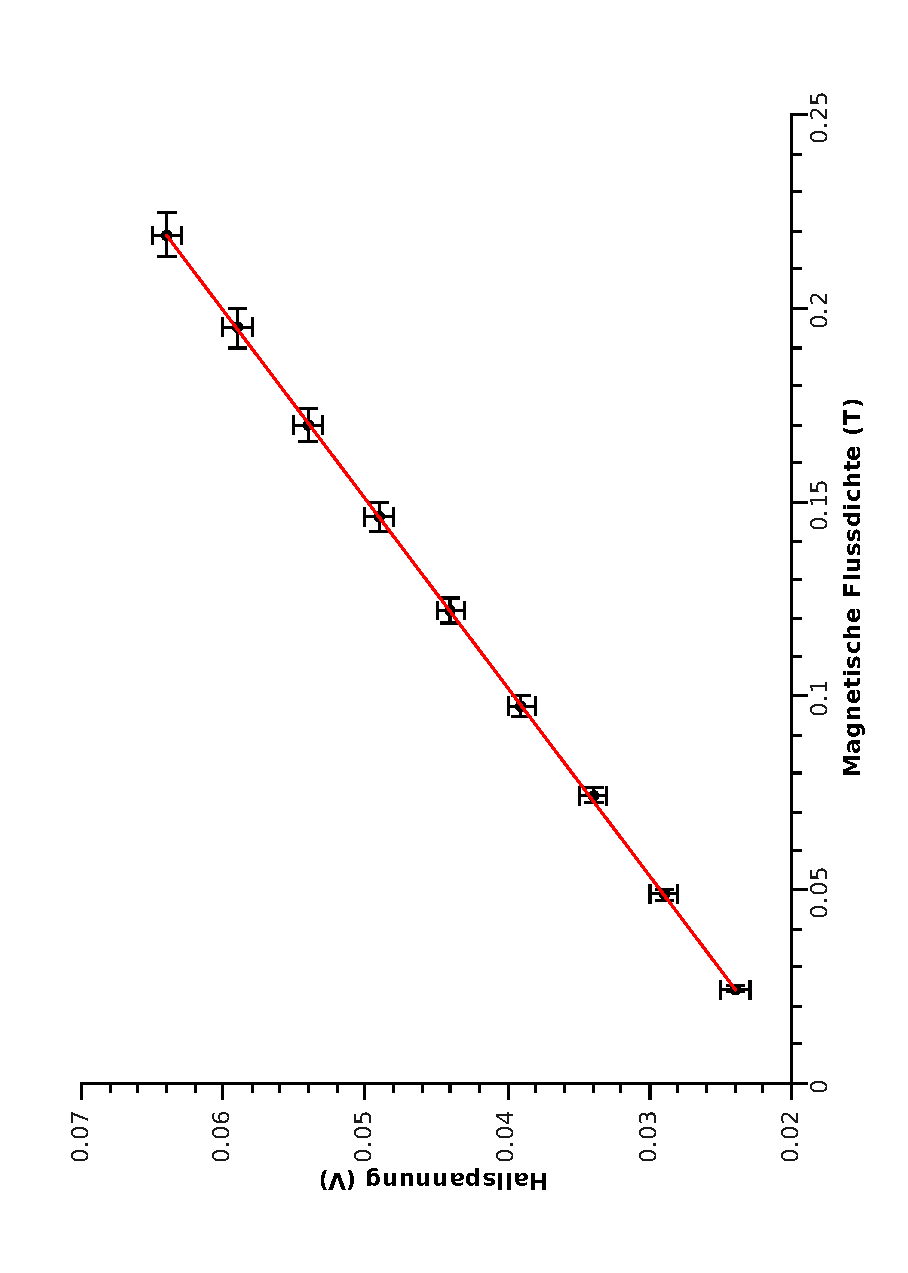
\includegraphics[width=0.9\linewidth, angle=-90]{npe.eps}
\caption{n-Ge}
\end{subfigure}
\begin{subfigure}{0.4\textwidth}
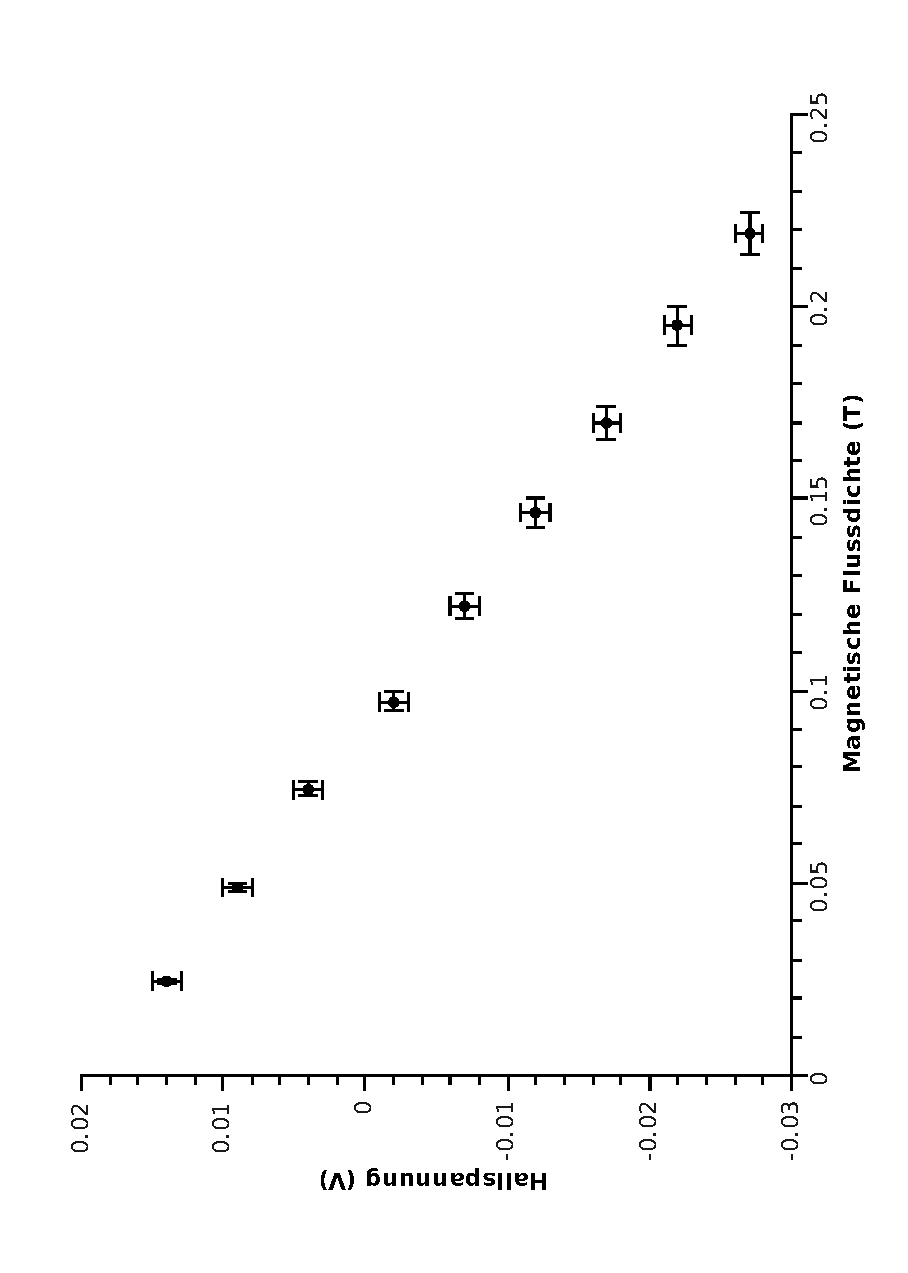
\includegraphics[width=0.9\linewidth, angle=-90]{npeumpol.eps}
\caption{n-Ge mit umgepoltem B-Feld}
\end{subfigure}
\\
\begin{subfigure}{0.4\textwidth}
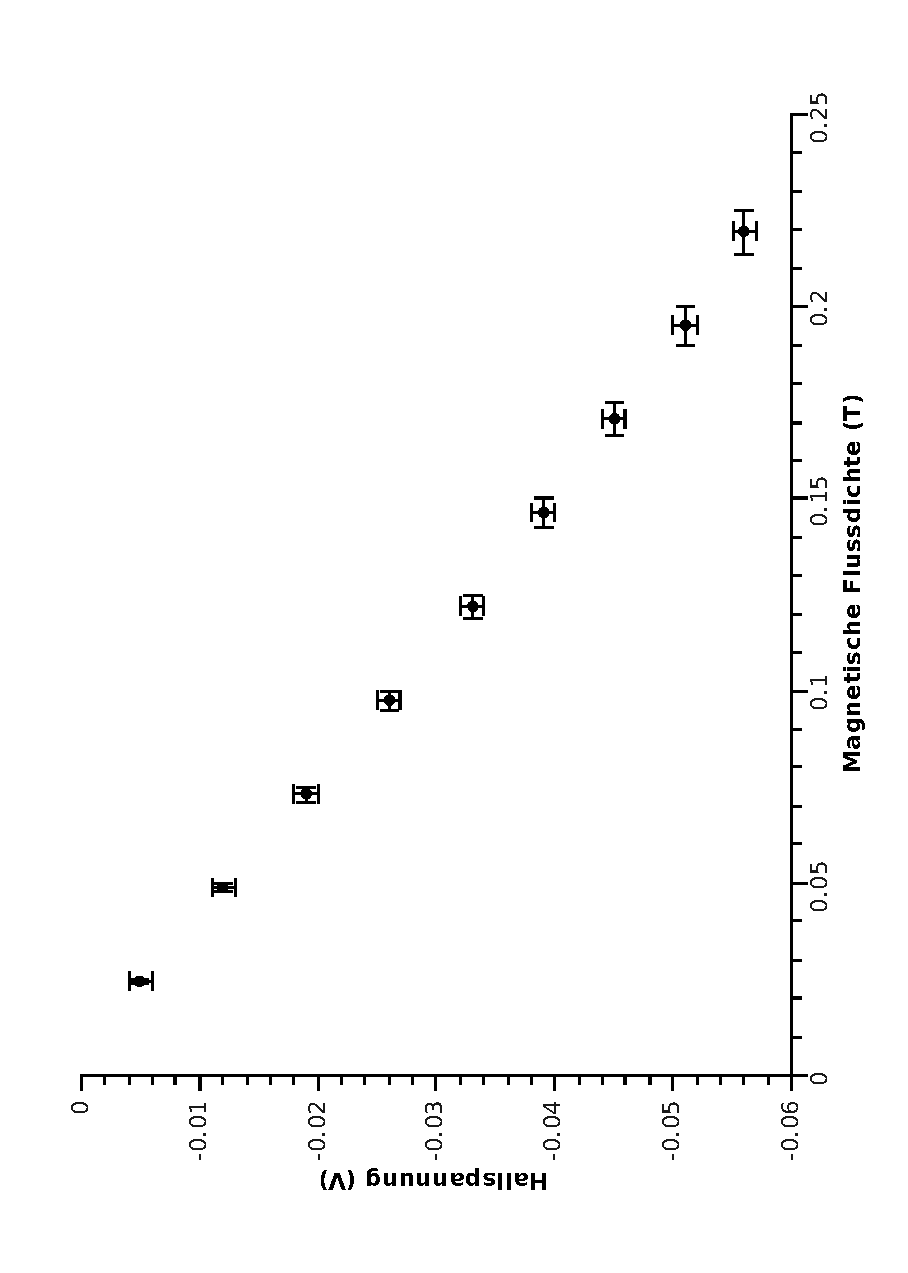
\includegraphics[width=0.9\linewidth, angle=-90]{ppe.eps}
\caption{p-Ge}
\end{subfigure}
\begin{subfigure}{0.4\textwidth}
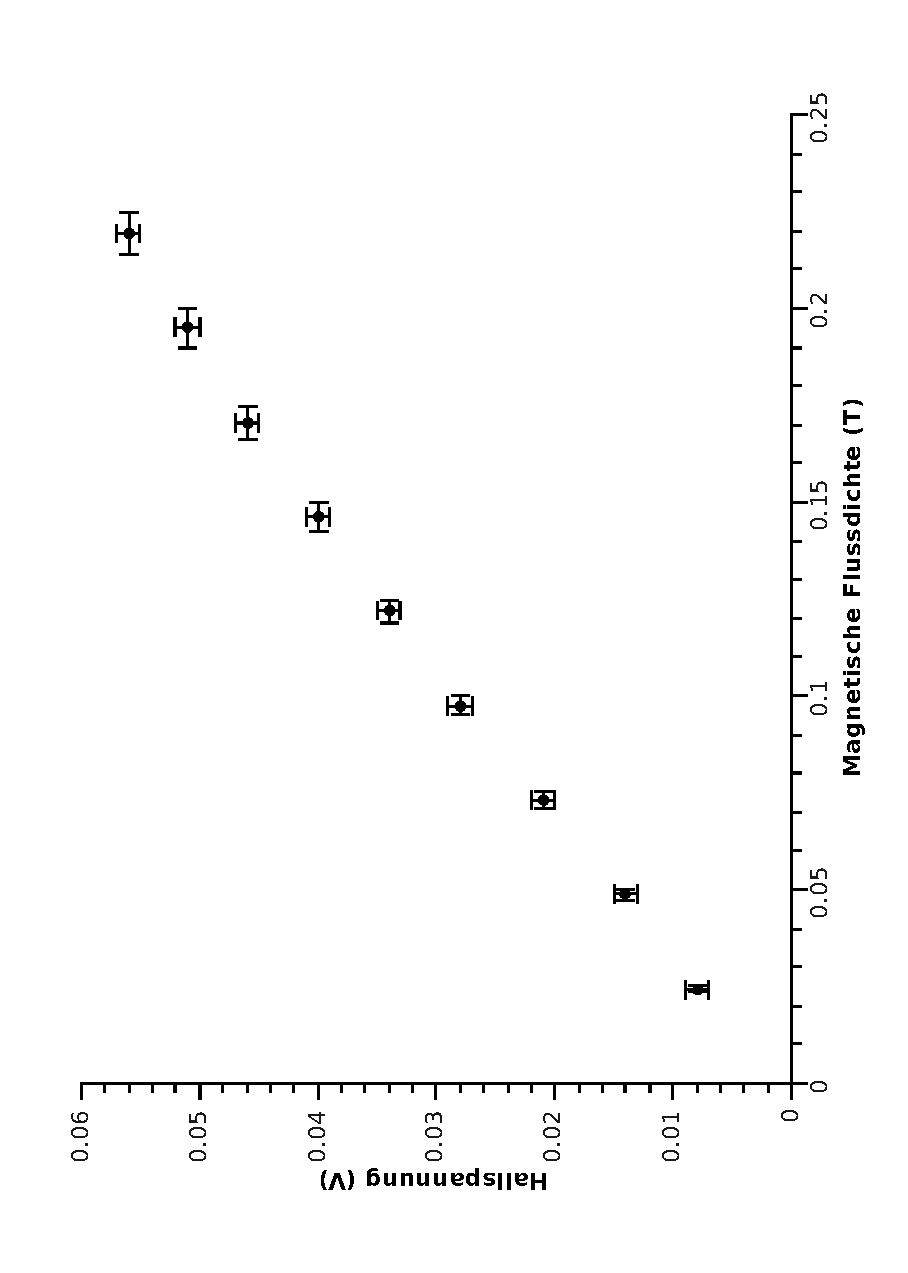
\includegraphics[width=0.9\linewidth, angle=-90]{ppeumpol.eps}
\caption{p-Ge mit umgepoltem B-Feld}
\end{subfigure}
\caption{Hallspannungen über B\label{hallbimg}}
\end{figure}



Da wir, in Übereinstimmung mit der Anleitung, bei der p-Ge Probe keine Messung der Längsspannung bei variiertem Probenstrom vorgenommen haben, können wir keine einfache Bestimmung ihres Widerstands vornehmen. Stattdessen haben wir die Längsspannung in Abhängigkeit des Magnetfelds geplotted und einen linearen Fit zu B=0 extrapoliert um eine Spannung für diesen Fall zu erhalten. Diese Spannung haben wir durch den konstanten Probenstrom von 0.025 A dividiert und einen Schätzwert für R erhalten:

$$ R_{p-Ge} = (58 \pm 3) \Omega $$

Um die Stichhaltigkeit des Verfahrens zu überprüfen haben wir die selbe Methode für die n-Ge Probe angewendet, deren Widerstand wir durch eine bessere Messung genauer kennen: $R_{n-Ge}=(43.3 \pm 0.5) \Omega$
Die Methode lieferte dabei $45.6 \Omega$, weswegen wir ihr vertrauen und nur die Unsicherheit auf $\pm 3 \Omega$ erhöhen.

Damit können wir den Magnetowiderstand an p-Ge bestimmen und auch die Beweglichkeit $\mu_p$ der Löcher in p-Ge.
\begin{figure}
\begin{subfigure}{0.4\textwidth}
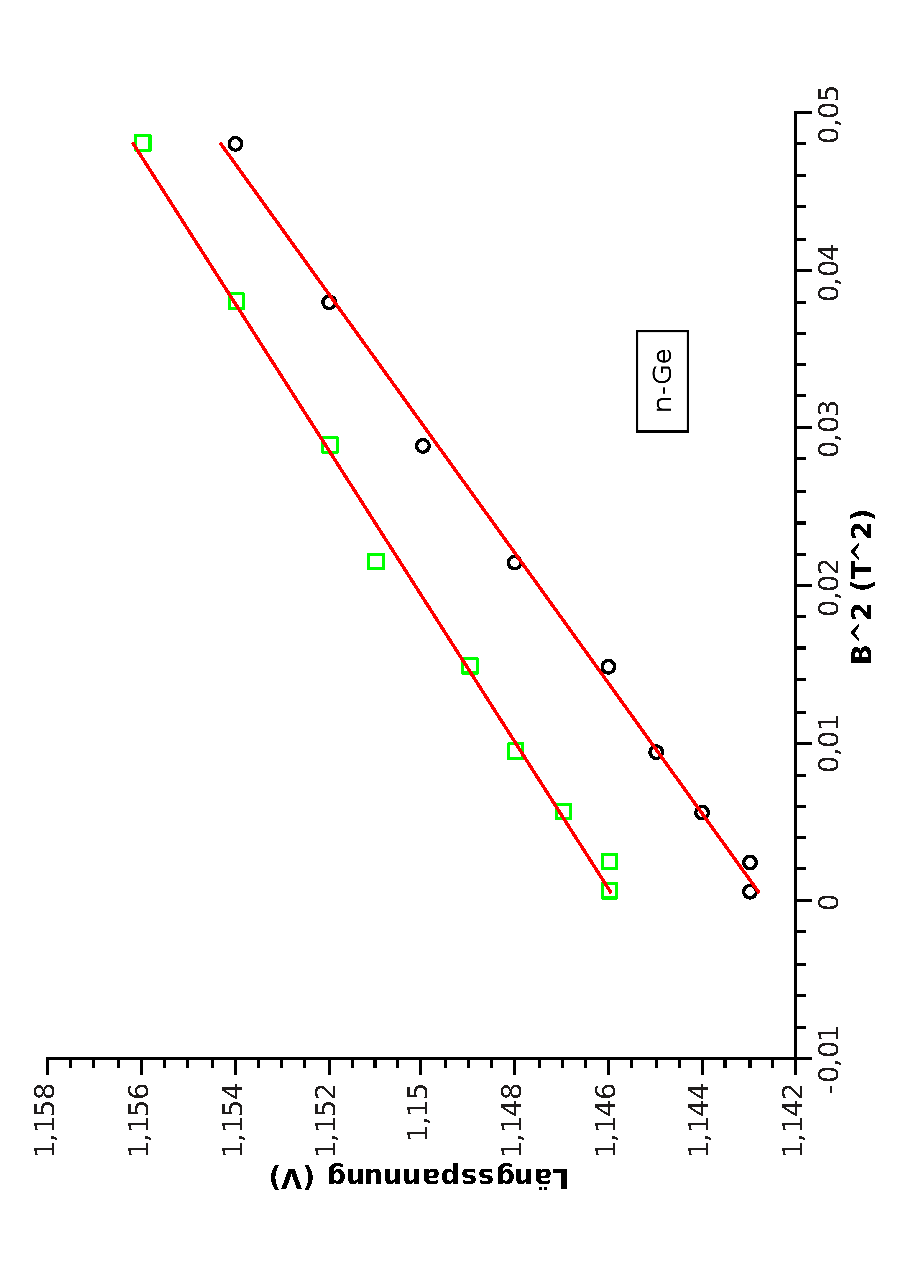
\includegraphics[width=0.9\linewidth, angle=-90]{magneton.eps}
\caption{Magnetowiderstand an n-Ge}
\end{subfigure}
\begin{subfigure}{0.4\textwidth}
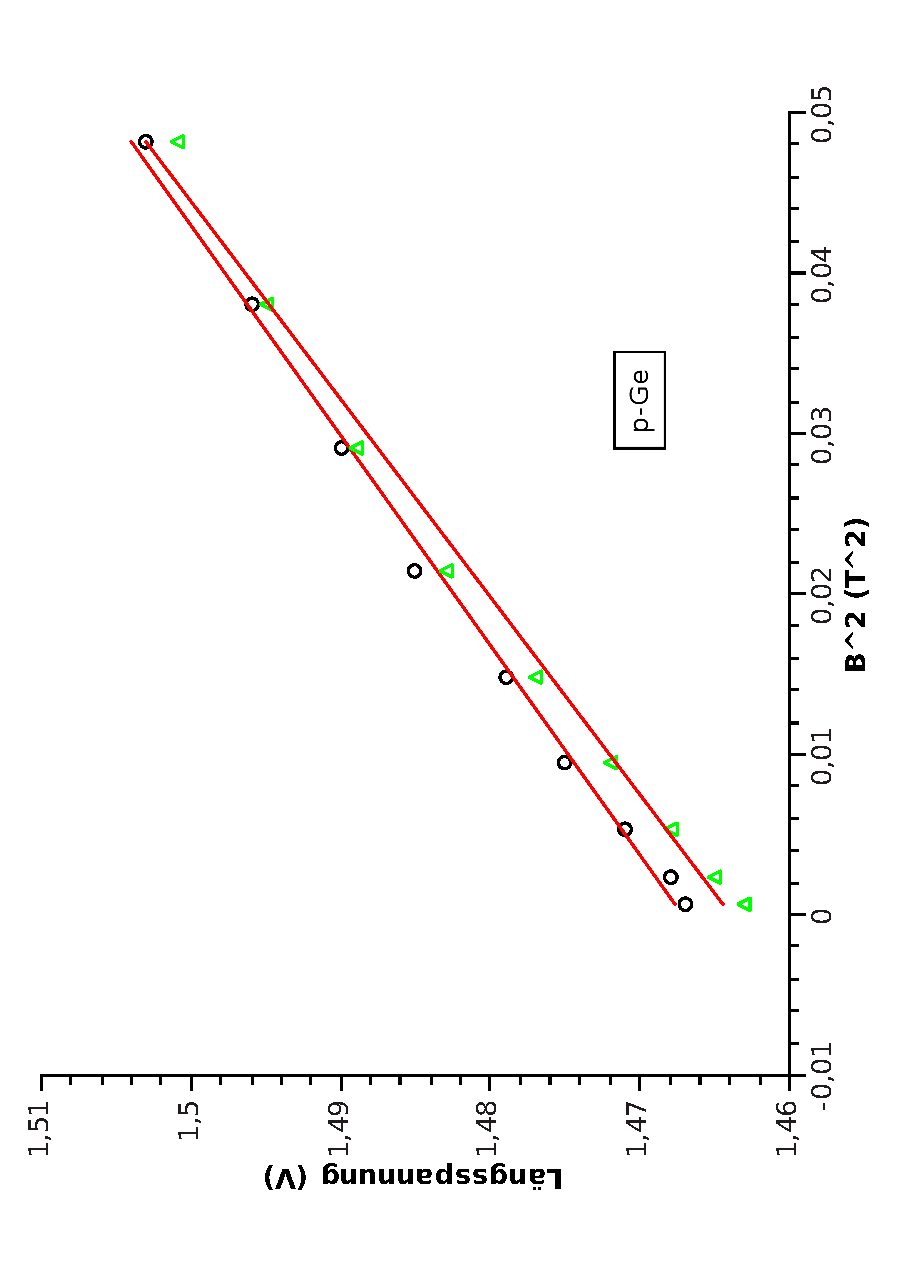
\includegraphics[width=0.9\linewidth, angle=-90]{magnetop.eps}
\caption{Magnetowiderstand an p-Ge}
\end{subfigure}
\caption{Längsspannung\label{magn} gegen $B^2$}
\end{figure}

\begin{figure}
\begin{subfigure}{0.4\textwidth}
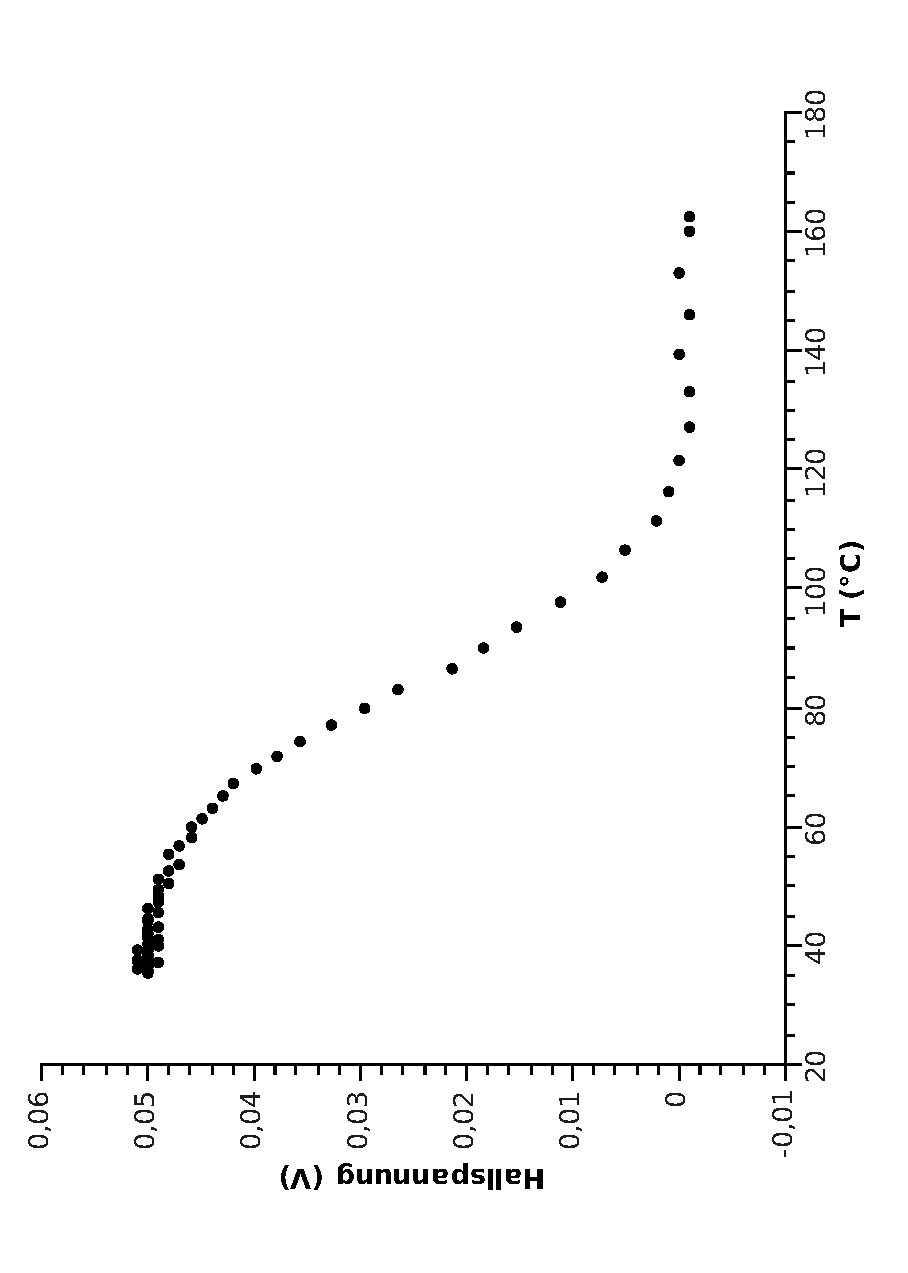
\includegraphics[width=0.9\linewidth, angle=-90]{temphall.eps}
\caption{Hallspannung}
\end{subfigure}
\begin{subfigure}{0.4\textwidth}
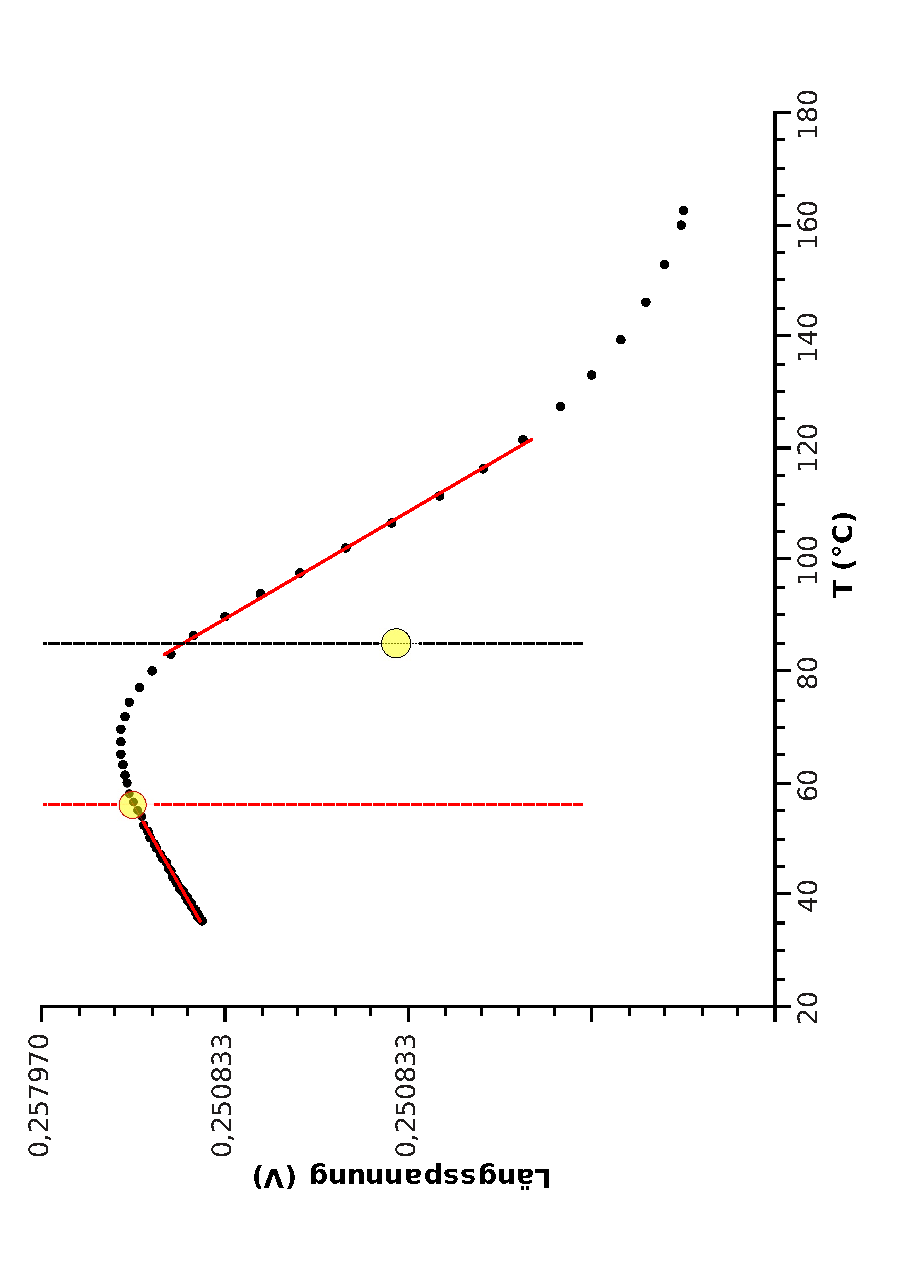
\includegraphics[width=0.9\linewidth, angle=-90]{templangs.eps}
\caption{\label{langssp}Längsspannung}
\end{subfigure}
\caption{Temperaturabhängigkeit an n-Ge}
\end{figure}



 
\section{Diskussion}		
\subsection*{Beweglichkeit}
Im Vergleich mit Literaturwerten zur Beweglichkeit von Ladungsträgern in Germanium sieht man eine gute Übereinstimmung mit unseren Ergebnissen: Das Taschenbuch der Physik von Stöcker nennt $\mu_n = 3900 \frac{cm^2}{Vs}$ für n-Ge und $\mu_p = 1900 \frac{cm^2}{Vs}$ für p-Ge. Das Ergebnis von $\mu_n = (0.38 \pm 0.03) \frac{m^2}{Vs}$ entspricht $\mu_n = (3800 \pm 300) \frac{cm^2}{Vs}$ und das von $\mu_p = (0.34 \pm 0.04) \frac{m^2}{Vs}$ entspricht $\mu_p = (3400 \pm 400) \frac{cm^2}{Vs}$. Dass wir bei der Beweglichkeit der Löcher so weit daneben liegen liegt am vereinfachten Modell, wenn wir zusätzlich die Beweglichkeit der Ladungsträger berücksichtigen, erhalten wir Werte von $\mu_n = (3600 \pm 300)$  und $\mu_p =(1900 \pm 400)$, was viel näher an den Literaturwerten liegt. 

Wir haben in "Festkörperphysik" von Siegfried Hunklinger übrigens noch Werte von 3800 und 1800 gefunden, die unseren noch näher kommen. Wir vertrauen daher Hunklinger.
\subsection*{Magnetowiderstände}								
Die Plots der relativen Magnetowiderstände in \textbf{Abb. (\ref{magn}) } gegen $B^2$ wurden so skaliert, dass sie gleiche absolute Bereiche von 0.03V	Größe zeigen, so dass sie direkt visuell verglichen werden können - und man sieht sofort am steileren Anstieg, dass der Widerstand von p-Ge größer ist.

Durch Auftragung der Längsspannung gegen das Quadrat der Magnetischen Flussdichte, wie das erweiterte Modell vorhersagt, erkennt man sofort den Magnetowiderstand: Die Werte liegen auf einer Geraden.

Aufgrund der Unsicherheiten der relativen Magnetowiderstände lässt sich keine verlässliche Aussage darüber machen, ob der Magnetowiderstand von der Orientierung des Magnetfeldes abhängt.

\subsection*{Erwärmung}
Durch Fits im Plot der Längsspannung in \textbf{Abb. (\ref{langssp})} erkennt man, dass bei der Erwärmung von 35°C auf ca. 70°C der Widerstand der Probe um 0.35 $\Omega$ zunimmt, während er von 80°C bis 120°C um 1 $\Omega$ abnimmt. Das bedeutet, dass auch $\rho$ diese Veränderungen durchmacht - und nachdem $\sigma$ der Kehrwert von $\rho$ ist, nimmt $\sigma$ ab, wo $\rho$ zunimmt, und $\sigma$ steigt, wo $\rho$ schwindet.

Von 35°C bis 70°C nimmt die $\sigma$ ab - von 80°C bis 120°C nimmt sie zu.

Nachdem die Hallspannung mit steigender Temperatur monoton sinkt, sinkt auch $R_H$ - das heißt, die Ladungsträgerkonzentration n nimmt wegen $R_H=\frac{1}{n\cdot q}$ ständig zu. 

Wegen $\mu= \frac{\sigma}{n\cdot q}$ sinkt die spezifische Leitfähigkeit $\sigma$ zwischen 35° und 70° stärker als die Konzentration n zunimmt - denn der Widerstand steigt in diesem Bereich, also muss die Beweglichkeit $\mu$ abnehmen. Im Bereich von 80° bis 120° sinkt der Widerstand aber, also muss $\mu$ wachsen, also muss $\sigma$ stärker wachsen als n abnimmt. 


Bei der Temperaturabhängigkeit sei noch erwähnt, dass die Hallspannung bei 160° auf etwa $\frac{1}{50}$ ihres ursprünglichen Wertes abfällt, während sich die Längsspannung nur etwa halbiert.

Wir konnten leider die Temperaturabhängigkeit der p-Ge Probe nicht untersuchen, da ihre Heizung nicht funktionierte. Hätten wir es tun können, hätten wir gesehen, dass sich bei ihr ein interessanter Effekt einstellt: das Vorzeichen der Hallspannung dreht sich ab einer gewissen Temperatur um, da irgendwann genug Elektronen in das Leiterband gehoben wurden, um die Anzahl der Löcher zu übertreffen und dann statt Elektronen- Löcherleitung stattgefunden hätte.


																								
\end{document}